\chapter*{Introduction}
\addcontentsline{toc}{chapter}{Introduction}

Visualization of the difference between two triangle meshes\footnotemark is often used in geometric morphometrics\footnotemark where the shapes of biological objects such as bones, facial symmetries and others are studied. In order to compare these objects, various difference metrics have been devised such as the distance between two overlaid meshes or the difference in curvature of corresponding parts of their surface. For demonstration and publication purposes it is extremely useful to visualize these difference metrics in such a way that they are easily understood. Presenting the differences on either raw triangle meshes or raw metric values is highly unsuggestive due to the large amount of data\footnotemark.

\addtocounter{footnote}{-3}
\stepcounter{footnote}\footnotetext{A triangle mesh is a collection of vertices, edges and triangles which is used for representing 3D objects in computer graphics.}
\stepcounter{footnote}\footnotetext{The word ``morphometrics'' is of Greek origin and means ``the quantitative analysis of form''.}
\stepcounter{footnote}\footnotetext{Triangle meshes used in this thesis have over 15,000 vertices and it is not uncommon for triangle meshes of regular objects to have over 100,000 vertices.}

We will first examine how visualizations are handled in publicly available software, mention their disadvantages and then we will state how we aim to improve them.

%%-----------------------------------------------------------------------------------------
%% SECTION
%%-----------------------------------------------------------------------------------------
\section*{Existing Mesh Difference Visualizations}
\label{sec:existing_visualizations}

Our main reference program will be Morphome3cs\footnotemark, a piece of software developed by researchers at Charles University which allows users to process and analyze 3D data, mostly of anthropological origin.

\footnotetext{\citet{Morpho}}

Morphome3cs is able to generate a homologous\footnotemark pair of triangle meshes from two arbitrary triangle meshes and use it to compute and visualize the difference between them. Currently, Morphome3cs is able to produce color-based visualizations of multiple difference metrics. These metrics are:

\footnotetext{Two triangle meshes are homologous if they have the same number of vertices, edges and triangles and there is a one-to-one mapping between them. Vertices are numbered and vertex \(v_i \in Mesh_1\) corresponds to vertex \(w_i \in Mesh_2\). Similarly for edges and triangles.}

\begin{itemize}
\item Corresponding vertex distance (Fig. \ref{fig:morpho_example})
\item Corresponding vertex distance projected into the surface normal
\item Angle between corresponding surface normals
\item FESA\footnotemark
\item Curvature difference
\end{itemize}

\footnotetext{Finite Element Surface Analysis - captures the difference between corresponding triangle areas}

The disadvantage of these color-based visualizations is that they fail to capture multidimensional information. For example, when using corresponding vertex distance as a metric, it is impossible to encode both its magnitude and its direction into color at the same time while maintaining visual clarity.

\begin{figure}[h]
\centering
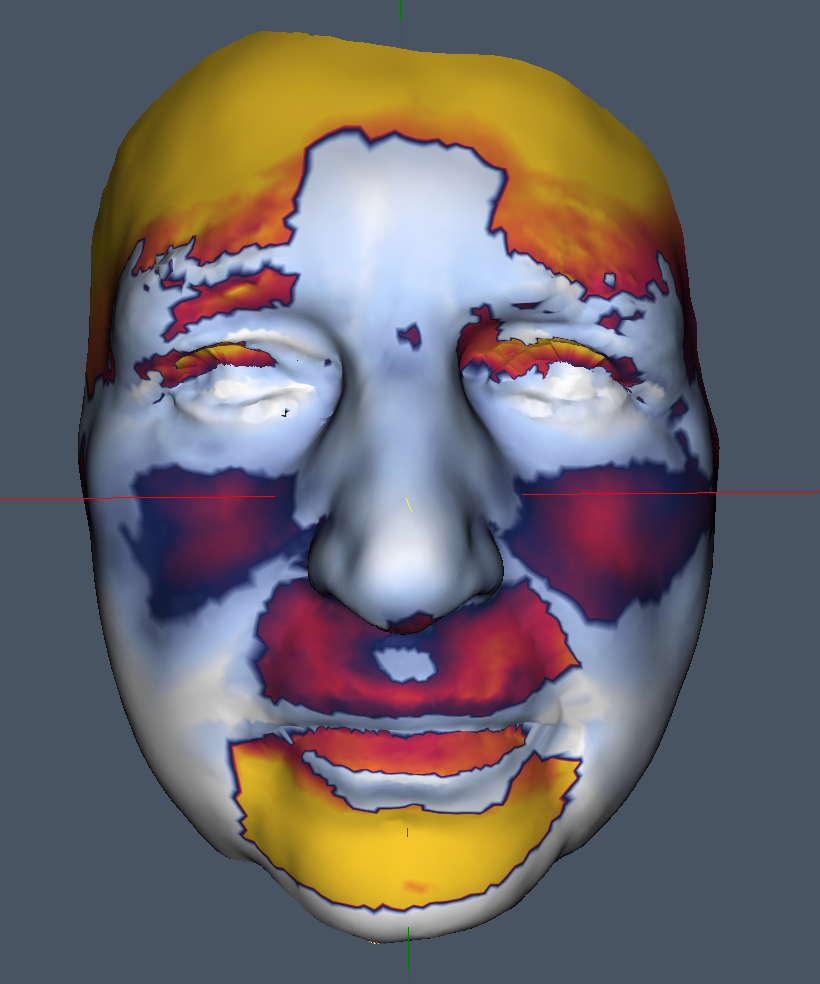
\includegraphics[width=0.5\textwidth]{./img/morpho-example01.PNG}
\caption[Morphome3cs - Vertex difference visualization]{Morphome3cs - Vertex difference visualization}
\label{fig:morpho_example}
\end{figure}

\begin{figure}[h]
\centering
	\begin{subfigure}{0.3\textwidth}
	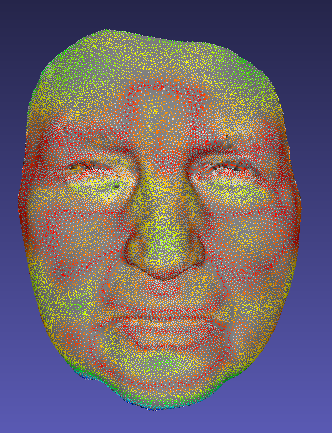
\includegraphics[width=\textwidth]{./img/meshlab-example01.PNG}
    \caption[MeshLab - Hausdorff Distance visualization]{MeshLab - Hausdorff Distance visualization}
    \label{fig:meshlab_example}
	\end{subfigure}
    \qquad
    \begin{subfigure}{0.3\textwidth}
	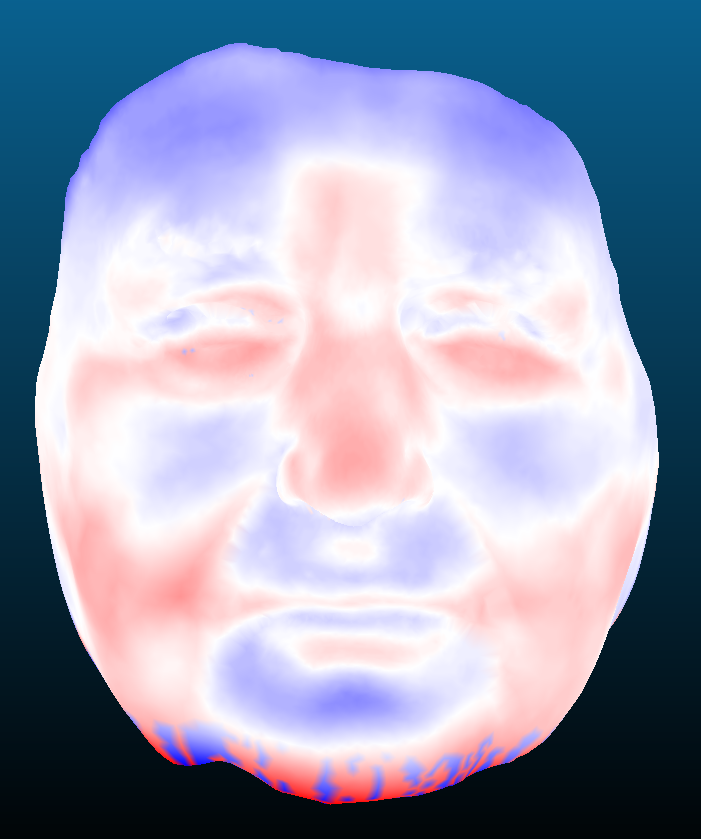
\includegraphics[width=\textwidth]{./img/cloudcompare-example01.PNG}
    \caption[CloudCompare - Vertex distance visualization]{CloudCompare - Vertex distance visualization}
    \label{fig:cloudcompare_example}
	\end{subfigure}
\caption{Visualizations in MeshLab and CloudCompare}
\end{figure}

Other approaches can be found for example in MeshLab \footnote{\citet{MeshLab}} (Fig. \ref{fig:meshlab_example}) or CloudCompare\footnote{\citet{CloudCmp}} (Fig. \ref{fig:cloudcompare_example}). In MeshLab, the difference between two arbitrary triangle meshes can be visualized directly without the homologization step using the Hausdorff Distance\footnotemark encoded into color. CloudCompare is also able to visualize the difference between two arbitrary triangle meshes (or even a triangle mesh and a point cloud or two point clouds). It does it by finding the nearest triangle to a given vertex, computing the distance between them and encoding this metric into color \citep{CloudCmpDistance}.

\footnotetext{One-sided Hausdorff Distance between two point sets \(S_1, S_2\) is defined as \(E(S_1, S_2) = \max_{p \in S_1} (\min_{p' \in S_2} d(p, p'))\) where \(d\) is the Euclidean distance between two points. Details of the computation used in MeshLab can be found in \citet{Metro98}.}

Another drawback of the presented visualizations is that they only capture local differences. This makes answering questions such as ``Which face has a larger nose?'' more difficult because the observer has to synthesize various local differences on their own. Such a method is then time-consuming and prone to inaccuracies.
%%-----------------------------------------------------------------------------------------
%% SECTION
%%-----------------------------------------------------------------------------------------
\section*{Our Goal}

In order to overcome the limitations of the above color-based visualizations, this thesis is looking to create an arrow-based visualization technique combined with clustering which will be able to display multidimensional information and also group similar information together automatically. As a proof of concept, we will apply it in various visualizations using the corresponding vertex distance metric because this metric suffers from information loss when visualized using colors. Other metrics which can be represented by arrows can be easily added. We will follow the approach applied in Morphome3cs, therefore our input will be two homologous triangle meshes. We will focus on the visual appearance of the devised visualizations and their implementation in an experimental application called MeshDiff. Lastly, a user study will be conducted to assess the quality of the new visualizations in various use cases. This study will serve as a basis for further development and potential incorporation of the visualizations into Morphome3cs.
%%-----------------------------------------------------------------------------------------
%% SECTION
%%-----------------------------------------------------------------------------------------
\section*{Thesis Structure}

Chapter 1 of this thesis is concerned with the description of the proposed visualizations and the main ideas behind them. Chapter 2 delves into the implementation details of the visualizations in MeshDiff. Chapter 3 provides user documentation of MeshDiff and chapter 4 presents the results of the user study.